\documentclass{article}
\usepackage[spanish]{babel}
\usepackage{graphicx}
\usepackage{float}
\usepackage{hyperref}

\title{\textbf{Introducción a Packet Tracer}}
\author{Lionel Cutró}
\date{\today}

\begin{document}
\maketitle

\section{Trabajo Práctico 1}
Consigan del trabajo:
Documentar su primera experiencia con el software de emulación Packet Tracer, haciendo incapié en las funcionalidades a utilizar durante la práctica.

\subsection{Packet Tracer}
Como principal vista sobre el software, podemos encontrar diferentes menús en la parte superior derecha, entre ellas; File, Edit, Options, View, Tools, Extensions, Window y Help.

Estos menús es algo estándar si se quiere decir, hay un punto importante que podemos destacar, en menú File, hay una opción llamada Open Samples, aquí podemos encontrar ejemplos de conexiones, que ya se encuentran armados y de los cuales podemos seleccionar y cargar en el software para verlo. Ejemplo podemos ver uno, Networking - FTP.

Además en Options - Preferences, podemos configurar un poco mas nuestra experiencia como usuario. Encontramos barras de herramientas, la primera podemos hallar acciones como deshacer, acercar y alejar, en la segunda barra, como encontrar; seleccionar objetos, eliminar objetos o incluso incluir algún objeto de dibujo.

Existe otra barra, que el la azul, donde tenemos dos botones "Lógico" y "Físico", en el Lógico, podemos ver como fluirán los datos a través de la red y la ilustración de como se conectan los dispositivos.

En la parte inferior, encontramos otra barra azul, donde hallamos otro par de iconos, como; Botón para encender/apagar todos los dispositivos, consiguiente veremos un botón de avance rápido (en tiempo), en el otro extremo veremos mas opciones, como; simulación y tiempo real, este ultimo es literal el tiempo actual donde las cosas ocurren, en simulación, podemos controlar el. En la parte inferior izquierda encontramos los componentes de red, donde podemos seleccionar enrutadores, ordenadores, etc, por ultimo en la parte inferior derecha encontramos el cuadro de escenario, aquí podemos crear paquetes de red para viajar a múltiples dispositivos y verlos durante el viaje.

\subsection{Dispositivos Finales}
En esta sección vamos a encontrar dispositivos "básicos" tal vez, que estos se encuentran en la parte inferior izquierda.
\begin{figure}[H]
    \centering
    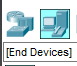
\includegraphics[width=0.15\linewidth]{end devices.PNG}
    \caption{Icono derecho - End Devices}
    \label{fig:enter-label}
\end{figure}

Aquí una vez hacemos el clic para ver las opciones, contiguo a la derecha, hay un panel que nos muestra varios dispositivos que corresponden a la categoría End Devices. Entre los mas comunes o acostumbrados de ver son; PC, Laptop, Impresora y Servidor.

Una vez seleccionado y arrastrados a la pantalla de trabajo, podemos visualizarlo y empezar a configurar si se necesita este dispositivo (haciend un clic en el icono del dispositivo en la pantalla de trabajo).
Ejemplo, la PC podemos jugar un poco con ella, y hacer modificaciones según sea necesario, ejemplo, cambio de placa de red, agregar/quitar micrófono y auriculares.
\begin{figure}[H]
    \centering
    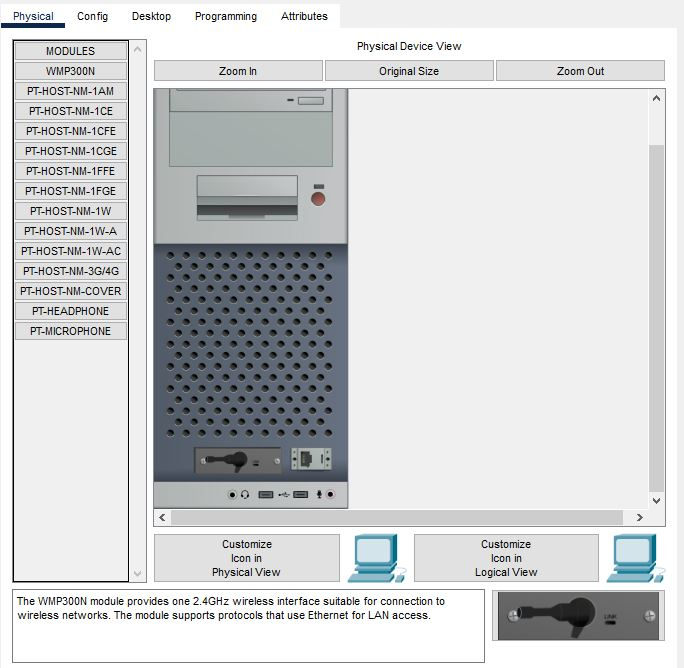
\includegraphics[width=0.70\linewidth]{Captura.JPG}
    \caption{Menú configuración PC}
\end{figure}

Esta misma lógica, o mecanismo sera igual para todos los dispositivos que queramos configurar a futuro, obviamente con la salvedad que las opciones de configuración varían según el dispositivo.

Importante destacar que el caso de la PC no es lo único que podemos configurar a nivel "hardware" además, podemos ingresar a la pestaña en la misma ventana a varias opciones, 'Desktop' podemos iniciar algunos programas de la PC, ejemplo; Terminal, navegador, firewall, entre otros, otras opciones mas, 'Programming', 'Config', 'Attributes'.

\subsection{Dispositivos de Red}
Esta sección vamos a encontrar los dispositivos 'Router' aquellos dispositivos de Red, lo vamos a ubicar también en la parte inferior izquierda en su botón dedicado.
\begin{figure}[H]
    \centering
    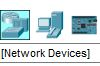
\includegraphics[width=0.25\linewidth]{lCaptura.JPG}
    \caption{Icono izquierdo - Network Devices}
\end{figure}
En la manera que seleccionamos anteriormente los dispositivos finales, es como vamos a seleccionar los Routers en esta sección, habrá varios tipos de routers de diferentes modelos.

Acá también vamos a poder configurar el router como podemos hacer con la PC anteriormente, cambiando los módulos del router, quitando o cambiando elementos del mismo. Respecto al resto de opciones de la misma ventana de configuración de modulos, vamos a encontrar 'CLI' esta pestaña nos muestra como el router bootea y se inicializa, y además nos brinda cierta información importante, ejemplo; la versión de IOS es importante saberlo, ya que esto nos marca las capacidades y caracteristicas del router con el cual estamos trabajando.

\begin{figure}[H]
    \centering
    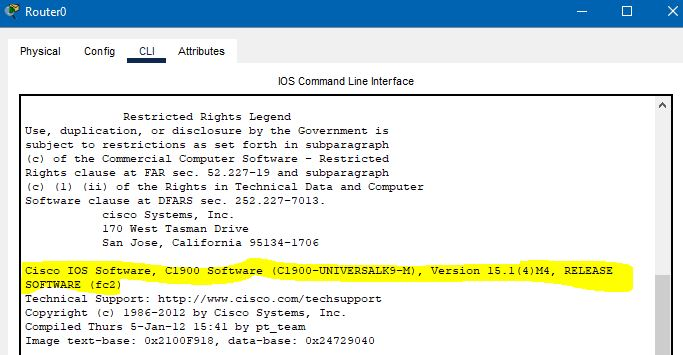
\includegraphics[width=0.75\linewidth]{cap1.JPG}
    \caption{Pestaña CLI - IOS -version}
\end{figure}

\subsection{Cableado}
En esta ultima sección, vamos a poder ver los tipos de cableado que existen en Paket Tracer, hay varios y cada uno de ellos dependen del tipo de conexión que queremos realizar.
AutoSelect; Esta opción nos habilita que al momento de realizar una conexión, nosotros elegimos los dispositivos y el software reconoce estos dispositivos y elige el cable correcto.
Consola; Este cable sirve para hacer conexiones PCs y Router para hacer uso de la consola.
USB; También podemos conectar PCs y Routers
Copper Straight Through; Sirve para hacer conexiones entre PCs, Switch y Routers, bajo estrictas reglas.
\subsection{Actividad Practica}
Esta conexión se realiza entre 2 PCs con un cable Cross Over, a su vez se configuran las PCs con sus IP correspondiente ejemplo; (192.168.1.1 y 192.168.1.2) luego en prompt console, se puede usar el comando ping 192.168.x.x para revisar que llegue la conexión a la otra pc.

Estudios posibles: Puedes observar la conectividad básica entre dispositivos, realizar pruebas de transferencia de datos, y ver cómo se comportan las redes simples sin un switch o router.

Limitaciones: Este tipo de conexión directa es limitada para redes más grandes o cuando se necesita conectar más de dos dispositivos. Estas limitaciones se superarán aprendiendo sobre switches, routers y otras técnicas de interconexión más avanzadas.

\bibliographystyle{plain}
\bibliography{}
Se utilizo el curso de introduccion dictado por Cisco
\href{https://github.com/lionelcutrocs}{GitHub}





\end{document}
